\section{Avaliação via simulação com dados reais}
\label{sec:sim}

Nesta seção avaliamos o \rmprt{} usando simulações dirigidas com dados
reais.  Utilizamos o mesmo conjunto de dados descrito na
\secstr~\ref{sec:char}.  Nosso foco é comparar o custo de remapear
mudanças de caminho usando o Paris traceroute com o custo de remapear
usando o \rmprt.

O custo de remapeamento usando o \rmprt{} varia de acordo com o salto
$s^\prime$ onde a mudança é detectada.  Calculamos o custo de
remapeamento do \rmprt{} para todos os saltos do caminho onde a mudança
pode ser detectada.  A \figstr~\ref{fig:sim.rmprt.start} mostra a
distribuição do custo de remapeamento de mudanças para o \rmprt{}.
Mostramos a distribuição dos custos mínimo, médio e máximo, calculados
sobre todos os saltos envolvidos em uma mudança.  Vemos que o custo
mínimo e máximo em geral são muito próximos.  Uma razão para este
comportamento é que várias mudanças de caminho envolvem poucos
roteadores, logo não existe muita variação em função do salto $s^\prime$
onde a mudança é detectada.  No resto deste artigo usaremos o custo
médio como representativo do custo de remapeamento com \rmprt{}.

\begin{figure}
\begin{center}
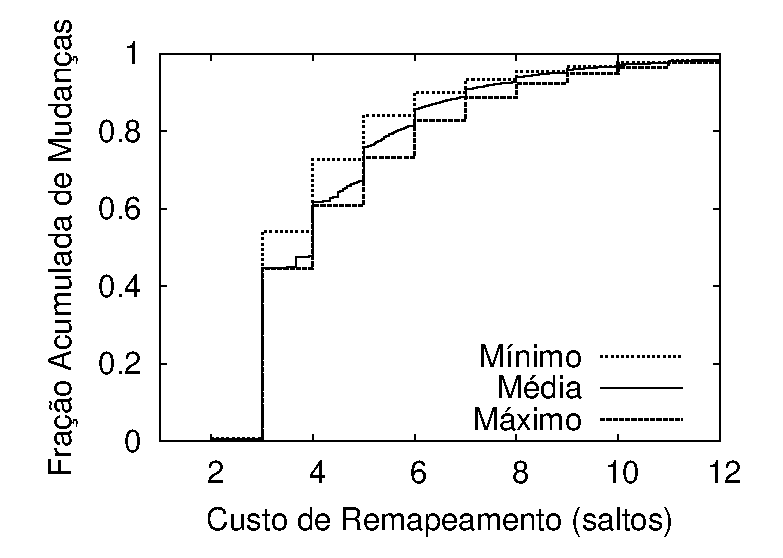
\includegraphics[width=0.47\textwidth]{figs/rmprtcost.eps}
\caption{Custo de remapeamento com \rmprt{} variando o salto
$\boldsymbol{s^\prime}$ de detecção da mudança.}
\label{fig:sim.rmprt.start}
\end{center}
\end{figure}

A \figstr~\ref{fig:sim.abs.cmp} compara o custo de remapeamento do
\rmprt{} com o custo de remapeamento do Paris traceroute.  Comparando
com a \figstr~\ref{fig:char.nrouters} vemos que o \rmprt{}
frequentemente precisa sondar um número de saltos maior do que o número
de saltos envolvidos numa mudança.  Este aumento deve-se a mudanças de
roteamento que precisam ser localizadas usando a técnica de pesquisa
binária antes de serem remapeadas.  Independente do processo de
localização, o \rmprt{} tem custo de remapeamento significativamente
menor que o do Paris traceroute.  Note que o custo de remapeamento do
\rmprt{} raramente é menor do que três saltos, mesmo com 9\% das
mudanças envolvendo apenas dois saltos
(\figstr~\ref{fig:char.nrouters}).  As mudanças que envolvem apenas dois
roteadores apenas removem saltos da rota antiga, e precisamos localizar
o salto onde a remoção aconteceu usando busca binária.  A busca binária
requer pelo menos três sondas a não ser que a mudança seja detectada nos
três primeiros saltos do caminho, o que acontece em 0,4\% das mudanças
em nossos dados.

\begin{figure}
\begin{center}
\subfigure[Custo de remapeamento]{
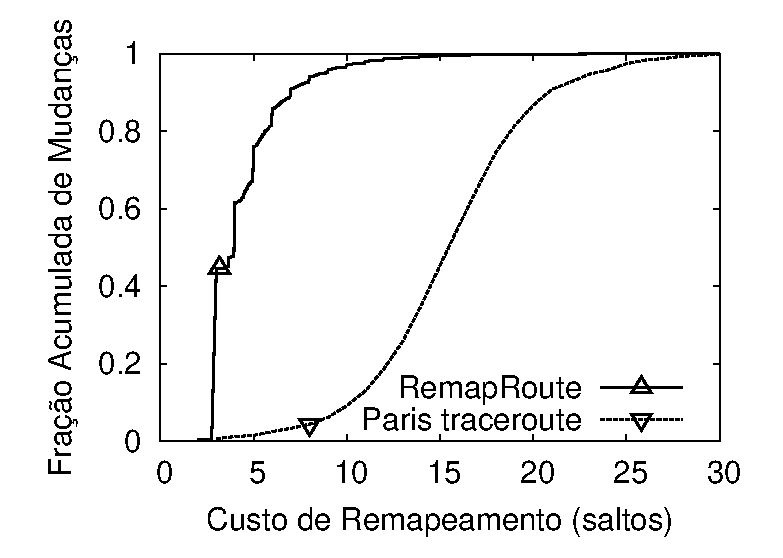
\includegraphics[width=0.47\textwidth]{figs/costcmp.eps}
\label{fig:sim.abs.cmp}}
\hspace{2mm}
\subfigure[Redução relativa do custo de remapeamento]{
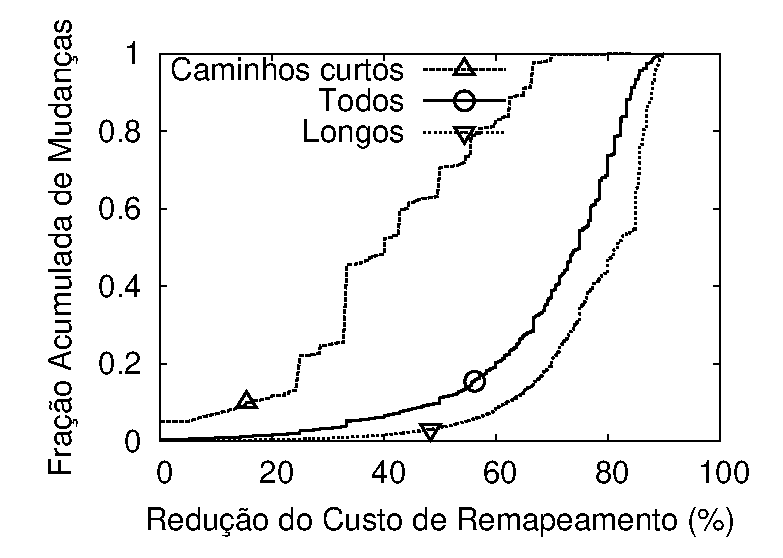
\includegraphics[width=0.47\textwidth]{figs/lensavings.eps}
\label{fig:sim.savings.cmp}}
\caption{Comparação do custo de remapeamento entre \rmprt{} e Paris
traceroute.}
\end{center}
\end{figure}

A \figstr~\ref{fig:sim.savings.cmp} mostra a distribuição da redução no
custo de remapeamento quando usamos \rmprt{} em vez do Paris traceroute.
Calculamos a redução do custo de remapeamento como $(C_\mathrm{Paris} -
C_\mathrm{\rmprt})/C_\mathrm{Paris}$, onde $C_\mathrm{Paris}$ é o número
de saltos remapeados pelo Paris traceroute e $C_\mathrm{\rmprt}$ é o
número de saltos remapeados pelo \rmprt{}.  A linha sólida, calculada
para todas as mudanças de caminho em nossos dados, mostra que a redução
no custo é significativa.  O \rmprt{} reduz pra menos da metade o custo
de remapeamento de 88\% das mudanças de caminho.  As linhas tracejadas
na \figstr~\ref{fig:sim.savings.cmp} mostram a redução no custo para
mudanças em rotas menores que 10 saltos (curtas) e maiores que 20 saltos
(longas).  Vemos que a redução no custo é mais acentuada para rotas
longas, onde o Paris traceroute desperdiça sondas em vários roteadores
que não estão envolvidos na mudança, e que o \rmprt{} traz redução de
custos para remapeamento mesmo em rotas curtas.

\subsection{Erros de remapeamento}

O \rmprt{} remapeia mudanças num caminho dado um salto $s^\prime$ onde
uma mudança foi detectada.  Isso pode levar a inconsistências caso um
caminho sofra duas ou mais mudanças disjuntas antes de detectarmos a
primeira mudança.  Por exemplo, um caminho $\{a, b, c, d, e, f, g\}$
pode mudar para $\{a, x, c, d, y, f, g\}$ entre duas medições
consecutivas com Paris traceroute.  Neste caso, podemos detectar duas
mudanças nos saltos $s^\prime = 1$ e $s^{\prime\prime} = 4$.
Infelizmente, dado $s^\prime$ ou $s^{\prime\prime}$, o \rmprt{}
remapeará apenas uma mudança.

Para avaliar a gravidade desse problema, a
\figstr~\ref{fig:sim.ndisjoint} mostra a distribuição do número de
mudanças disjuntas para os pares de medições consecutivas dos caminhos
em nosso conjunto de dados.\footnotemark{}  Vemos que 79\% das medições
consecutivas remapeiam apenas uma mudança disjunta, que o \rmprt{}
remapeará corretamente para qualquer salto $s^\prime$ onde a mudança for
detectada.  Apenas 3\% das medições consecutivas remapeiam três ou mais
mudanças disjuntas, indicando que o \rmprt{} remapeará a nova rota
corretamente na maioria dos casos.

\footnotetext{No nosso conjunto de dados só medimos caminhos com Paris
traceroute quando uma mudança é detectada.  Todos os pares de medições
consecutivas remapeiam pelo menos uma mudança disjunta.}

\begin{figure}
\begin{center}
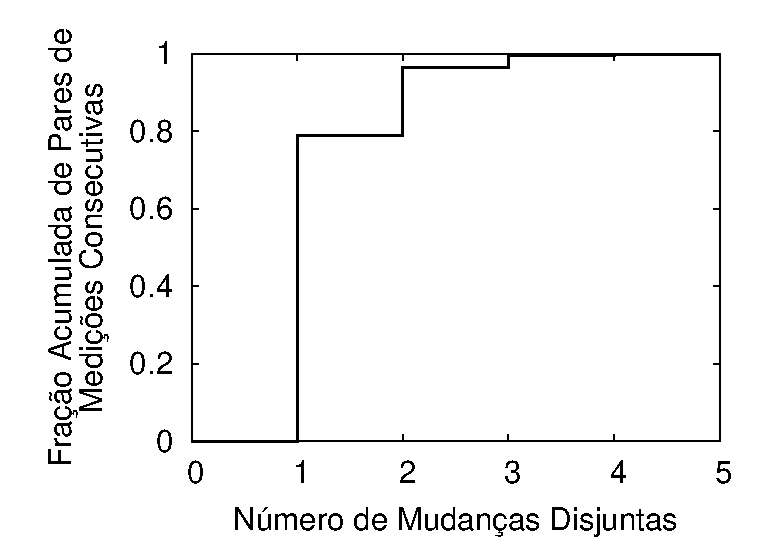
\includegraphics[width=0.47\textwidth]{figs/ndisjoint.eps}
\caption{Distribuição do número de mudanças disjuntas entre duas
medições com Paris traceroute.}
\label{fig:sim.ndisjoint}
\end{center}
\end{figure}

Três outros fatores contribuem para minimizar o impacto de mudanças
disjuntas.  Primeiro, o \rmprt{} pode remapear mudanças disjuntas
anteriores ao salto de detecção $s^\prime$ caso ele as detecte durante o
processo de remapeamento.  Em particular, a probabilidade do \rmprt{}
remapear uma mudança disjunta anterior ao salto de detecção $s^\prime$
no nosso conjunto de dados é 43\%.  Segundo, uma mudança disjunta que
não for remapeada quando executarmos \rmprt{} será detectada e remapeada
no futuro (assumindo que o processo de sondagem para detecção de
mudanças de caminho seja capaz de detectar todas as mudanças possíveis).
Qualquer mudança disjunta que não for remapeada causa apenas uma
inconsistência temporária nos dados.  Terceiro, a redução do custo de
remapeamento obtida com \rmprt{} pode ser utilizada para aumentar a
frequência de sondagem para detecção de mudanças e reduzir a chance de
ocorrerem duas mudanças em um caminho antes de detectarmos a primeira.

Outra limitação do \rmprt{} é que o mecanismo de busca binária pode
falhar quando a ordem relativa de dois saltos se inverte da rota antiga
para a nova rota.  Um exemplo extremo, mas ilustrativo, é uma mudança de
$C(t_{i-1}) = \{a, b, c, d, e, f\}$ para $C(t) = \{a, e, d, c, b, f\}$.
Apenas 0,9\% das mudanças de caminho em nossos dados invertem a ordem
relativa de saltos.  Como inversão da ordem relativa de saltos é um
evento raro, tomamos a decisão conservadora de remapear o caminho por
inteiro (como o Paris traceroute) quando uma inversão é detectada
durante o processo de remapeamento.  Como mostram os resultados
anteriores, essa limitação não compromete a utilidade do \rmprt{}.
